\documentclass[a4paper, 12pt]{article}
\usepackage[utf8]{inputenc}
\usepackage{xcolor}
\usepackage{graphicx}

\title{Delivery - Esercizio}
\author{Simone Pozzebon}
\date{February 2021}

\begin{document}

\maketitle Un gruppo di ragazzi, per guadagnare dei soldi, decide di organizzare un servizio di consegna di ciboa domicilio pertanto si accorda con dei ristoranti per poter consegnare a casa i pasti che sono statiordinati via web dai loro clienti. Tutto il servizio viene organizzato via web.Un cliente che desidera comprare dei pasti pronti e che questi gli vengano consegnati a casa, sicollega al sito web, sceglie il ristorante fra un elenco, sceglie i piatti, la loro quantità, paga con lacarta di credito (o con un altro mezzo di pagamento), indica l’indirizzo (l’indirizzo di consegna nondeve essere troppo distante) e attende la consegna a casa.Il prezzo dei pasti è comprensivo di un ricarico che spetta al servizio di delivery, non serve vengaconosciuto dal cliente finale, ma deve essere possibile calcolarlo in modo che parte del ricavato vadaimmediatamente conteggiato e versato su conto del servizio delivery. Saranno il servizio delivery ed isingoli ristoranti che fisseranno l’importo che spetta al servizio di trasporto.

\subsection{Testo}
Un gruppo di ragazzi, per guadagnare dei soldi, decide di organizzare un servizio di consegna di ciboa domicilio pertanto si accorda con dei ristoranti per poter consegnare a casa i pasti che sono statiordinati via web dai loro clienti. Tutto il servizio viene organizzato via web.Un cliente che desidera comprare dei pasti pronti e che questi gli vengano consegnati a casa, sicollega al sito web, sceglie il ristorante fra un elenco, sceglie i piatti, la loro quantità, paga con lacarta di credito (o con un altro mezzo di pagamento), indica l’indirizzo (l’indirizzo di consegna nondeve essere troppo distante) e attende la consegna a casa.Il prezzo dei pasti è comprensivo di un ricarico che spetta al servizio di delivery, non serve vengaconosciuto dal cliente finale, ma deve essere possibile calcolarlo in modo che parte del ricavato vadaimmediatamente conteggiato e versato su conto del servizio delivery. Saranno il servizio delivery ed isingoli ristoranti che fisseranno l’importo che spetta al servizio di trasporto.

\subsection{Cosa fare}
\begin{itemize}
    \item Un cliente deve essere in grado di ordinare un piatto.
    \item Un ristorante deve essere in grado di preparare i piatti.
    \item Un ristorante deve in ogni momento essere in grado di conoscere i ricavi del ristorante e della delivery.
    \item Un servizio di delivery deve essere in grado di ritirare e consegnare a domicilio i piatti.
\end{itemize}

\subsection{Modello Concettuale}
\begin{enumerate}
    \item \textit{Piatto:} venduto da un qualsiasi ristorante, collegato a esso c'e' il costo e disponibilita'.
    \item \textit{Distinta base:} rappresenta la ricetta del piatto.
    \item \textit{Prodotto:} elemento composto della distinta base.
    \item \textit{Componente:} ingrediente primario della distinta base.
    \\
    \item \textbf{Ristorante:} ristorante.
    \item \textbf{Rider:} fattorini per il ristorante.
    \item \textbf{Utenti:} clienti del ristorante per ordinare in presenza.
    \item \textbf{Menu:} rappresenta il menu' dei piatti del ristorante.
    \\
    \item \underline{Cliente:} clienti dell'applicazione per ordinare da remoto.
    \item \underline{Trasporto:} indica il codice relativo al fattorino e ordini legati a esso.
    \item \underline{Ordine:} collegato al menu', rappresenta il piatto ordinato.
    \\
    \item \textcolor{green}{Utente}: cliente del ristorante secondo il sistema di pagamento.
    \item \textcolor{green}{Operazione:} transazione del pagamento.
    \item \textcolor{green}{Account}: indica piu' operazioni legati all'account collegati all'operazione.
    
    \subsection{Schema Concettuale}
    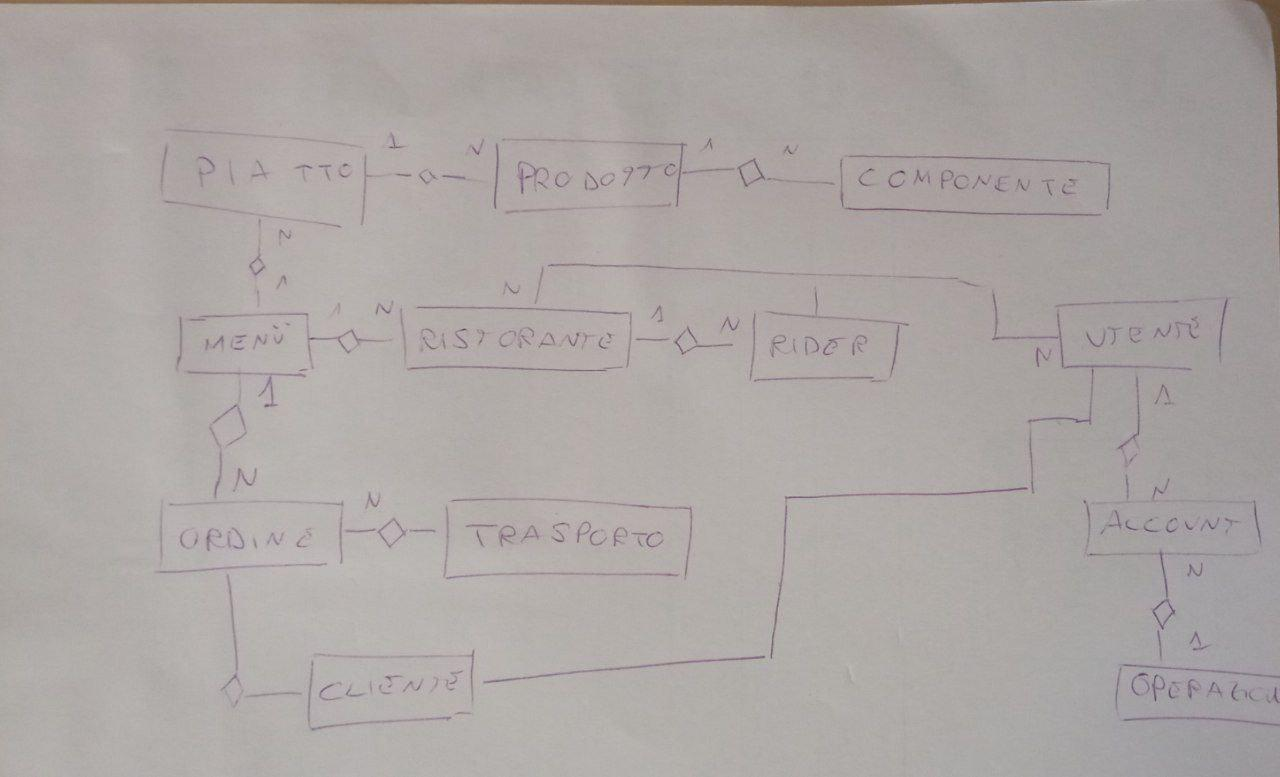
\includegraphics[width=15cm]{photo_2021-02-02_21-29-01.jpg}
    
\end{enumerate}
\end{document}

